\documentclass{article}
\usepackage[utf8]{inputenc}
\usepackage{polski}
\usepackage{fancyhdr} % Required for custom headers
\usepackage{lastpage} % Required to determine the last page for the footer
\usepackage{extramarks} % Required for headers and footers
\usepackage[usenames,dvipsnames]{color} % Required for custom colors
\usepackage{graphicx} % Required to insert images
\usepackage{listings} % Required for insertion of code
\usepackage{courier} % Required for the courier font
\usepackage[onelanguage]{algorithm2e}
\usepackage{pgfplots}
\pgfplotsset{width=10cm,compat=1.9}
\usepgfplotslibrary{external}

% Margins
\topmargin=-0.45in
\evensidemargin=0in
\oddsidemargin=0in
\textwidth=6.5in
\textheight=9.0in
\headsep=0.25in
\usepackage{tikz}
\usetikzlibrary{calc}
\linespread{1.1} % Line spacing

% Set up the header and footer
\pagestyle{fancy}
\lhead{\hmwkAuthorName} % Top left header
\chead{\hmwkClass\ \hmwkTitle} % Top center head
\rhead{\firstxmark} % Top right header
\lfoot{\lastxmark} % Bottom left footer
\cfoot{} % Bottom center footer
\rfoot{Strona\ \thepage\ z\ \protect\pageref{LastPage}} % Bottom right footer
\renewcommand\headrulewidth{0.4pt} % Size of the header rule
\renewcommand\footrulewidth{0.4pt} % Size of the footer rule

\setlength\parindent{0pt} % Removes all indentation from paragraphs
%----------------------------------------------------------------------------------------
%	DOCUMENT STRUCTURE COMMANDS
%	Skip this unless you know what you're doing
%----------------------------------------------------------------------------------------

% Header and footer for when a page split occurs within a problem environment
\newcommand{\enterProblemHeader}[1]{
}

% Header and footer for when a page split occurs between problem environments
\newcommand{\exitProblemHeader}[1]{
\nobreak\extramarks{#1 (continued)}{#1 continued on next page\ldots}\nobreak
\nobreak\extramarks{#1}{}\nobreak
}

\setcounter{secnumdepth}{0} % Removes default section numbers
\newcounter{homeworkProblemCounter} % Creates a counter to keep track of the number of problems

\newcommand{\homeworkProblemName}{}
\newenvironment{homeworkProblem}[1][Zadanie \arabic{homeworkProblemCounter}]{ % Makes a new environment called homeworkProblem which takes 1 argument (custom name) but the default is "Problem #"
\stepcounter{homeworkProblemCounter} % Increase counter for number of problems
\renewcommand{\homeworkProblemName}{#1} % Assign \homeworkProblemName the name of the problem
\section{\homeworkProblemName} % Make a section in the document with the custom problem count
\enterProblemHeader{\homeworkProblemName} % Header and footer within the environment
}{
\exitProblemHeader{\homeworkProblemName} % Header and footer after the environment
}

\newcommand{\problemAnswer}[1]{ % Defines the problem answer command with the content as the only argument
\noindent\framebox[\columnwidth][c]{\begin{minipage}{0.98\columnwidth}#1\end{minipage}} % Makes the box around the problem answer and puts the content inside
}

\newcommand{\homeworkSectionName}{}
\newenvironment{homeworkSection}[1]{ % New environment for sections within homework problems, takes 1 argument - the name of the section
\renewcommand{\homeworkSectionName}{#1} % Assign \homeworkSectionName to the name of the section from the environment argument
\subsection{\homeworkSectionName} % Make a subsection with the custom name of the subsection
\enterProblemHeader{\homeworkProblemName\ [\homeworkSectionName]} % Header and footer within the environment
}{
\enterProblemHeader{\homeworkProblemName} % Header and footer after the environment
}

%----------------------------------------------------------------------------------------
%	NAME AND CLASS SECTION
%----------------------------------------------------------------------------------------

\newcommand{\hmwkTitle}{Lista nr 4} % Assignment title
\newcommand{\hmwkDueDate}{Niedziela, 10 Grudnia 2017} % Due date
\newcommand{\hmwkClass}{OBLICZENIA NAUKOWE} % Course/class
\newcommand{\hmwkAuthorName}{Tymoteusz Surynt} % Your name
\renewcommand*\contentsname{Podsumowanie}

%----------------------------------------------------------------------------------------
%	TITLE PAGE
%----------------------------------------------------------------------------------------

\title{
\vspace{2in}
\textmd{\textbf{\hmwkClass:\ \hmwkTitle}}\\
\normalsize\vspace{0.1in}\small{\hmwkDueDate}\\
\vspace{3in}
}

\author{\textbf{\hmwkAuthorName}}
\date{Numer indeksu: 229794} % Insert date here if you want it to appear below your name

%----------------------------------------------------------------------------------------

\begin{document}

\maketitle

%----------------------------------------------------------------------------------------
%	TABLE OF CONTENTS
%----------------------------------------------------------------------------------------

%\setcounter{tocdepth}{1} % Uncomment this line if you don't want subsections listed in the ToC

\newpage
\tableofcontents
\newpage

%----------------------------------------------------------------------------------------
%	PROBLEM 1
%----------------------------------------------------------------------------------------

% To have just one problem per page, simply put a \clearpage after each problem

\begin{homeworkProblem}
%opis problemu
\subsection{Opis problemu}
Celem zadania było stworzenie funkcji, która będzie w stanie wyliczać ilorazy różnicowe dla zadanej funkcji.
%opis rozwiązania
\subsection{Opis rozwiązania}
\begin{algorithm}[H]
 \SetKwInput{KwData}{Dane}
 \KwData{
 \\x - tablica zawierająca wartości węzłów $x_0, x_1, x_2,\ldots$
 \\
 f - tablica zawierająca wartości funkcji $f(x_0), f(x_1),\ldots$
 }
 \SetKwInput{KwResult}{Wynik}
 \KwResult{
	fx – wektor długości $n + 1$ zawierający obliczone ilorazy różnicowe\\
 }
 \SetKwInput{TitleOfAlgo}{Funkcja}
 \TitleOfAlgo{ilorazyRoznicowe(x::Vector{Float64}, f::Vector{Float64})}
 $size \leftarrow length(x)$\;
 $output[size]$\;
 \For{$i$ in $1:size$}{
 	$output[i] \leftarrow f[i]$\;
 }
 \For{$i$ in $1:size$}{
 	$j \leftarrow size$\;
 	\While{$j>i$}{
 		$output[j] \leftarrow \frac{output[j]-output[j-1]}{x[j]-x[j-i]}$\;
 		$j \leftarrow j-1$\;
	 }
 }
	\KwRet{$output$}

  
 \caption{Ilorazy Różnicowe}
\end{algorithm}
\vspace{3mm}
Powyższy algorytm opiera się na własności iloczynu różnicowego: $f[x_0,x_1,x_2,\ldots,x_n]=\frac{f[x_1,x_2,\ldots,x_n]-f[x_0,x_1,\ldots,x_{n-1}]}{x_n-x_0}$ z której łatwo da się zauważyć, że kolejny iloczyn można szybko wyliczyć mając poprzedni. Jako, że wszystkie iloczyny są zapisywane w tablicy, dostęp do poprzednich nie jest problemem, jednak każda zmiana przy wyliczeniu iloczynu powoduje szereg zmian w następnych iloczynch. Żeby to poprawić występuje druga pętla, while, które umożliwia poprawianie wyników. Zmiany istnieją, ponieważ $f[x_1,x_2,\ldots,x_n]$ jest wyliczane na bieżąco.\\

%wyniki
\subsection{Testy}
Testy dla powyższej funkcji były przeprowadzane w następujący sposób:
wartości uzyskane przez funkcje były porównywane do prawdziwych, pamiętając o dokładności obliczeń, która wynosiła: $10.0^{-5}$. Aby zdać test, funkcja musiała być w odległości dokładności od prawdziwego wyniku.
\begin{enumerate}
\item Test 1:$$ilorazyRoznicowe([1.0,2.0,3.0,4.0,5.0,6.0,7.0],[-1.0,-5.0,2.0,3.0,0.3,0.2,0.6])$$
Wynik właściwy:
 $$[-1.0, -4.0, 5.5, -2.83333, 0.804167, -0.1275, 0.00402778]$$
Wynik otrzymany:
 $$[-1.0, -4.0, 5.5, -2.83333, 0.804167, -0.1275, 0.00402778]$$
 Test zdany
 \item Test 2:$$ilorazyRoznicowe([1.0,10.0,20.0,30.0,40.0,50.0,60.0],[-1.202,111.0,-4.44122,12.0,-0.3222113,0.15,10.3])$$
Wynik właściwy:
 $$[-1.202, 12.4668888889, -1.26374, 0.0663155, -0.00238692, 0.0000659068, 0]$$
Wynik otrzymany:
 $$[-1.202, 12.4669, -1.26374, 0.0663155, -0.00238692, 6.59068e-5, -1.46576e-6]$$
 Test zdany
  \item Test 3:$$ilorazyRoznicowe([3.0,1.0,5.0,6.0],[1.0,-3.0,2.0,4.0])$$
Wynik właściwy:
 $$[1.0, 2.0, -0.375, 0.175]$$
Wynik otrzymany:
 $$[1.0, 2.0, -0.375, 0.175]$$
 Test zdany
\end{enumerate}

\end{homeworkProblem}
%----------------------------------------------------------------------------------------
%	PROBLEM 2
%----------------------------------------------------------------------------------------

\begin{homeworkProblem}
%opis problemu
\subsection{Opis problemu}
Celem zadania było stworzenie funkcji, która będzie w stanie wyliczać wartości wielomianu interpolacyjnego n-tego stopnia
w postaci Newtona, dla podanego punktu.
%opis rozwiązania
\subsection{Opis rozwiązania}
\begin{algorithm}[H]
 \SetKwInput{KwData}{Dane}
 \KwData{
 \\x - tablica zawierająca wartości węzłów $x_0, x_1, x_2, \ldots$\\
 fx -  tablica zawierająca wartości ilorazów różnicowych $f(x_0), f(x_0,x_1),\ldots$\\
 $t$ - punkt dla którego liczymy wartość wielomianu\\
 }
 \SetKwInput{KwResult}{Wynik}
 \KwResult{
	nt – wartość wielomianu w punkcie t\\
 }
 \SetKwInput{TitleOfAlgo}{Funkcja}
 \TitleOfAlgo{warNewton (x::Vector{Float64}, fx::Vector{Float64}, t::Float64)}
	$size \leftarrow length(x)$\;
	$reszta \leftarrow fx[size]$\;
	$i \leftarrow size-1$\;
	\While{$i>0$}{
		$reszta \leftarrow reszta*(t-x[i])+fx[i]$\;
		$i \leftarrow i-1$\;
	}
	\KwRet{$reszta$}
 \caption{Algorytm Hornera dla wielomianu w postaci Newton}
\end{algorithm}
\vspace{3mm}
Powyższy algorytm działa w myśl uogólnionego algorytmu Hornera, jednak uwzględnia postać Newtona. Pierwsza wartość (w tym wypadku znajduje się na końcu tablicy, ponieważ ta postać zakłada, że największa potęga znajduje się na końcu) zostaje bez zmian, kolejne uzyskuje się przez dodanie do współczynika z oryginalnej funckji, poprzedniej wartości pomnożonej przez różnicę miejsca w którym szukamy wartości i wartości $x_i$ (dla normlanego wielomianu byłoby po prostu t). Ostatnia wartość jak i w algorytmie Hornera jest poszukiawną wartością.
%wyniki
\subsection{Testy}
Testy dla powyższej funkcji były przeprowadzane w następujący sposób:
wartości uzyskane przez funkcje były porównywane do prawdziwych, pamiętając o dokładności obliczeń, która wynosiła: $10.0^{-5}$. Aby zdać test, funkcja musiała być w odległości dokładności od prawdziwego wyniku.
\begin{enumerate}
\item Test 1:$$warNewton([1.0,2.0,3.0,4.0,5.0,6.0,7.0],[-1.0,-5.0,2.0,3.0,0.3,0.2,0.6],3.0)$$
Wynik właściwy:
 $$-7.0$$
Wynik otrzymany:
 $$-7.0$$
 Test zdany
 \item Test 2:$$warNewton([1.0,10.0,20.0,30.0,40.0,50.0,60.0],[-1.202,111.0,-4.44122,12.0,-0.3222113,0.15,10.3],5.0)$$
Wynik właściwy:
 $$-121622826.79285003$$
Wynik otrzymany:
 $$-1.2162282679285003e8$$
 Test zdany
  \item Test 3:$$warNewton([3.0,1.0,5.0,6.0],[1.0,-3.0,2.0,4.0],3.0)$$
Wynik właściwy:
 $$1.0$$
Wynik otrzymany:
 $$1.0$$
 Test zdany
\end{enumerate}
\end{homeworkProblem}
%----------------------------------------------------------------------------------------
%	PROBLEM 3
%----------------------------------------------------------------------------------------

% To have just one problem per page, simply put a \clearpage after each problem

\begin{homeworkProblem}
%opis problemu
\subsection{Opis problemu}
Celem zadania było stworzenie funkcji, która będzie w stanie znajdować współczyniki wielomianu interpolacyjnego w postaci Newtona.
%opis rozwiązania
\subsection{Opis rozwiązania}
\begin{algorithm}[H]
 \SetKwInput{KwData}{Dane}
 \KwData{
 \\x - tablica zawierająca wartości węzłów $x_0, x_1, x_2,\ldots$\\
 fx -  tablica zawierająca wartości ilorazów różnicowych $f(x_0), f(x_0,x_1),\ldots$\\
 
 }
 \SetKwInput{KwResult}{Wynik}
 \KwResult{
	a - wektor zawierający obliczone współczynniki postaci naturalnej\\
 }
 \SetKwInput{TitleOfAlgo}{Funkcja}
 \TitleOfAlgo{naturalna (x::Vector{Float64}, fx::Vector{Float64})}
 $size \leftarrow length(x)$\;
 $a[size] \leftarrow fx[size]$\;
 $i \leftarrow size-1$\;
 \While{$i>0$}{
 	$a[i] \leftarrow fx[i]$\;
 	\For{$j$ in $i:size-1$}{
 		$a[j] \leftarrow a[j]-x[i]*a[j+1]$\;
 	}
 	$i \leftarrow i-1$\;
 }
 \KwRet{$a$}
 \caption{Współczynniki postaci naturalnej}
\end{algorithm}
\vspace{3mm}

%wyniki
\subsection{Testy}
Testy dla powyższej funkcji były przeprowadzane w następujący sposób:
wartości uzyskane przez funkcje były porównywane do prawdziwych, pamiętając o dokładności obliczeń, która wynosiła: $10.0^{-5}$. Aby zdać test, funkcja musiała być w odległości dokładności od prawdziwego wyniku.
\begin{enumerate}
\item Test 1:$$naturalna([3.0,1.0,5.0,6.0],[1.0, 2.0, -0.375, 0.175])$$
Wynik właściwy:
 $$[-8.75, 7.525, -1.95, 0.175]$$
Wynik otrzymany:
 $$[-8.75, 7.525, -1.95, 0.175]$$
 Test zdany
 \item Test 2:$$naturalna([1.0,1.0,2.0,3.0,4.0,5.0,6.0],[-1.2,1.0,-4.2,1.0,-0.33,0.5,10.3])$$
Wynik właściwy:
 $$[1213.62, -4001.19, 5083.39, -3167.19, 1024.17, -164.3, 10.3]$$
Wynik otrzymany:
 $$[1213.62, -4001.19, 5083.39, -3167.19, 1024.17, -164.3, 10.3]$$
 Test zdany
  \item Test 3:$$naturalna([1.0,7.0,2.0,0.20,1.0,0.022,0.02],[-1.2,0.20,-3.2,11.0,-2.33,0.9,1.7])$$
Wynik właściwy:
 $$[-186.73928, 335.83764, -172.67936, -8.99048, 47.84888, -18.1774, 1.7]$$
Wynik otrzymany:
 $$[-186.73928, 335.83764, -172.67936, -8.99048, 47.84888, -18.1774, 1.7]$$
 Test zdany
\end{enumerate}


\end{homeworkProblem}
%----------------------------------------------------------------------------------------
%	PROBLEM 4
%----------------------------------------------------------------------------------------

% To have just one problem per page, simply put a \clearpage after each problem

\begin{homeworkProblem}
%opis problemu
\subsection{Opis problemu}
Celem zadania było stworzenie funkcji, która będzie w stanie rysować wykresy dla wielomianu interpolacyjnego i podanej funkcji.
%opis rozwiązania
\subsection{Opis rozwiązania}
\begin{algorithm}[H]
 \SetKwInput{KwData}{Dane}
 \KwData{
 \\f - funkcja dla, której rysujemy wykres\\
 $a,b$ - przedział interpolacji\\
 n - stopień wielomianu interpolacyjnego\\
 [GlobalPrec- precyzja wykresu (zmienna globalna, standardowo ustawiona na 100)]
 }
 \SetKwInput{KwResult}{Wynik}
 \KwResult{
	Wykres z zaznaczonymi funkcjiami
 }
 \SetKwInput{TitleOfAlgo}{Funkcja}
 \TitleOfAlgo{rysujNnfx(f,a::Float64,b::Float64,n::Int)}
 $prec \leftarrow \frac{b-a}{n}$\;
 $x[n+1]$\;
 $fx[n+1]$\;
 \For{$i$ in $0:n$}{
 	$x[i+1] \leftarrow a+i*prec$\;
 	$fx[i+1] \leftarrow f(x[i+1])$\;
 }
 $fn \leftarrow ilorazyRoznicowe(x, fx)$\;
 $outputFun[GlobalPrec]$\;
 $outputInt[GlobalPrec]$\;
 $array[GlobalPrec]$\;
 $prec \leftarrow \frac{b-a}{GlobalPrec}$\;

 \For{$i$ in $0:GlobalPrec$}{
	 $t \leftarrow a+i*prec$\;
 	 $outputInt[i+1] \leftarrow warNewton(x,fn,t)$\;
 	 $outputFun[i+1] \leftarrow f(t)$\;
 	 $array[i+1] \leftarrow t$\;
 }
 plot(array,[outputFun , outputInt], label=["Wynik dla funkcji" "Wynik dla interpolacji"])
 \vspace{3mm}
 \caption{Rysowanie wykresów funkcji}
\end{algorithm}
\vspace{3mm}
Powyższa funkcja w pierwszej kolejności dzieli przedział na ilość węzłów interpolacji aby punkty były równomiernie rozrzucone i   wylicza $x_0,x_1,\ldots$ oraz wartości funkcji w tych punktach. Dla wcześniej obliczonych danych wykonuje fukcję opisaną w Zadaniu 1, która oblicza ilorazy różnicowe. Następnie przygotowuje dwie tablice w których będą zapisywane wyniki pod wyświetlanie ich na wykresie. Po wyliczeniu kroku co który będą wyliczane wartości, wykonuje się pętla w której owe wartości są wyliczane. Dla wielomianu interplacyjnego są one wyliczane funcją z Zadania 2. Na sam koniec uzyskane wyniki są prezentowane na wykresie używając pakietu Plots i Plotly.
%wyniki
\subsection{Testy}
W tym przypadku przeprowadzenie testów było bardzo trudne, a odpowiednie testy na bardziej zaawanoswoanych przykładach będą przeprowadzane w zadaniu 5 i 6, więc w tej części porównam tylko czy wykres funkcji (nie wielomianu) podanej przez naszą funkcje będzie podobny do takiego narysowanego przez niezależny program do generownania wykresów.
\begin{center}
	Wykres wykonany przez naszą funkcję:\\
	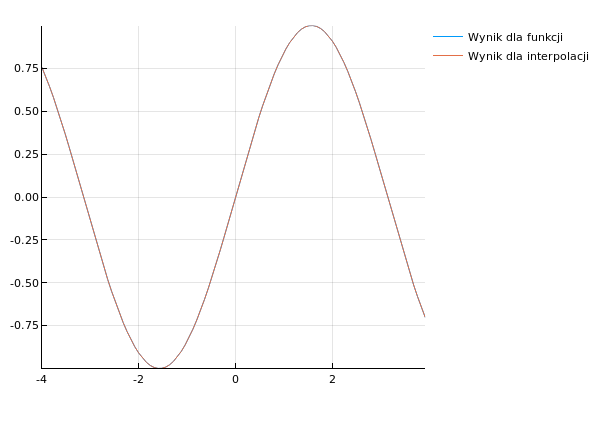
\includegraphics[scale=0.5]{sinx.png}\\
	Wykres z FooPlot.com:\\
	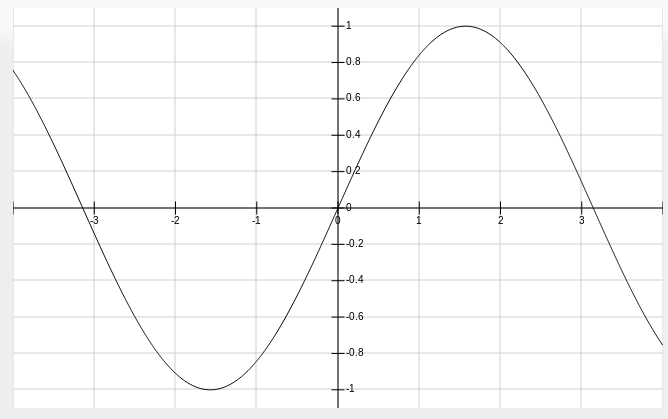
\includegraphics[scale=0.5]{sinxfoo.png}\\
\end{center}
Widzimy, że wykresy są podobne, więc nasza funkcja poprawnie rysuje wykresy funkcji.
\end{homeworkProblem}
\clearpage
%----------------------------------------------------------------------------------------
%	PROBLEM 5
%----------------------------------------------------------------------------------------

% To have just one problem per page, simply put a \clearpage after each problem

\begin{homeworkProblem}
%opis problemu
\subsection{Opis problemu}
Zadanie polegało na narysowaniu wykresów poprzez skorzystanie z funkcji napisanej w Zadaniu 4 dla podanych przypadków:
\begin{enumerate}
\item $e^x$, [0,1], n= 5, 10, 15
\item $x^2sin(x)$, [-1,1], n= 5, 10, 15
\end{enumerate}
%opis rozwiązania
\subsection{Opis rozwiązania}
Korzystam z uprzednio napisanej funckji poprzez uruchomienie jej z podanymi parametrami.
%wyniki
\subsection{Wyniki}
\begin{center}
Wynik dla podpunktu 1. z n=5\\
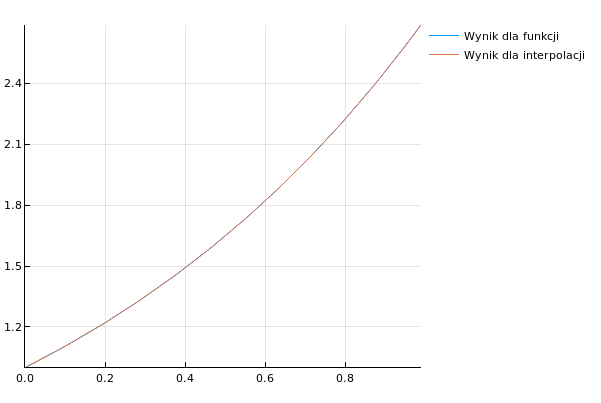
\includegraphics[scale=0.5]{5/a5.png}\\
Wynik dla podpunktu 1. z n=10\\
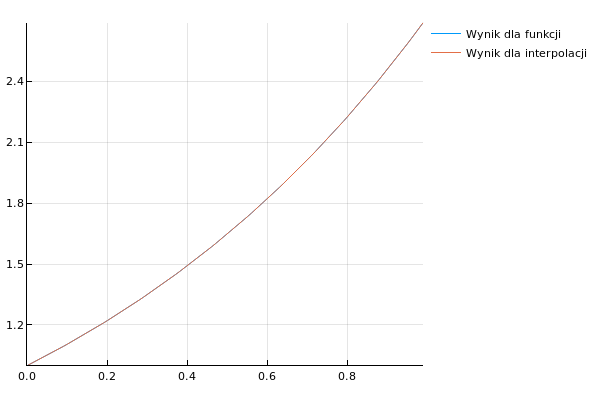
\includegraphics[scale=0.5]{5/a10.png}\\
Wynik dla podpunktu 1. z n=15\\
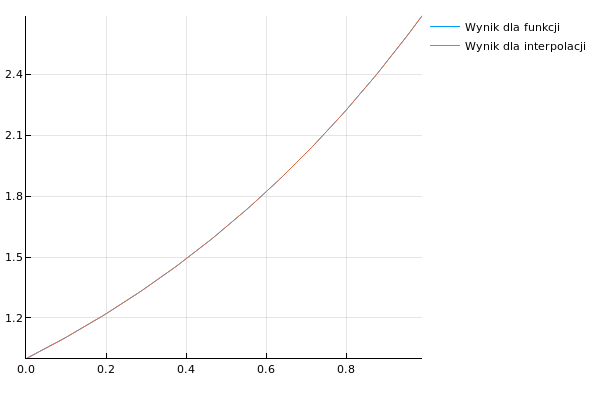
\includegraphics[scale=0.5]{5/a15.png}\\
Wynik dla podpunktu 2. z n=5\\
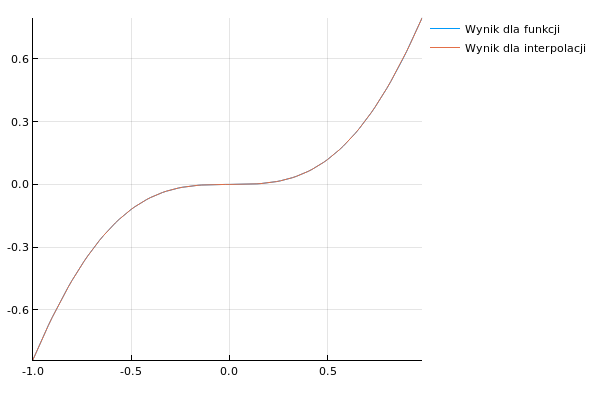
\includegraphics[scale=0.5]{5/b5.png}\\
Wynik dla podpunktu 2. z n=10\\
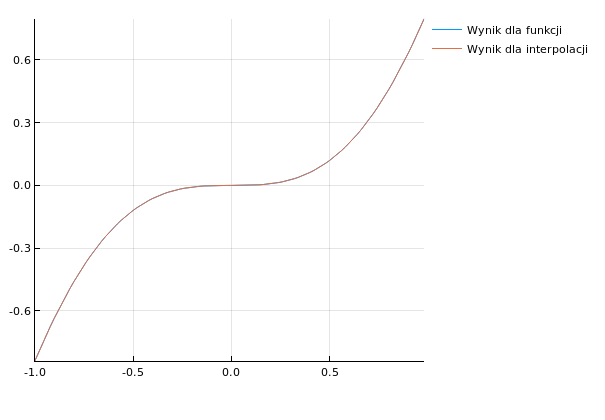
\includegraphics[scale=0.5]{5/b10.png}\\
Wynik dla podpunktu 2. z n=15\\
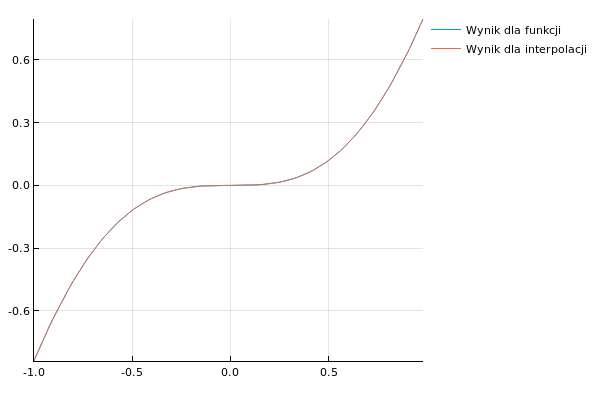
\includegraphics[scale=0.5]{5/b15.png}\\
\end{center}

%wnioski
\subsection{Wnioski}
Łatwo da się zauważyć, że oba wykresy funkcji są do siebie bardzo zbliżone i nawet jeśli różnice istnieją to są ona pomijalnie miałe.\\
\begin{center}
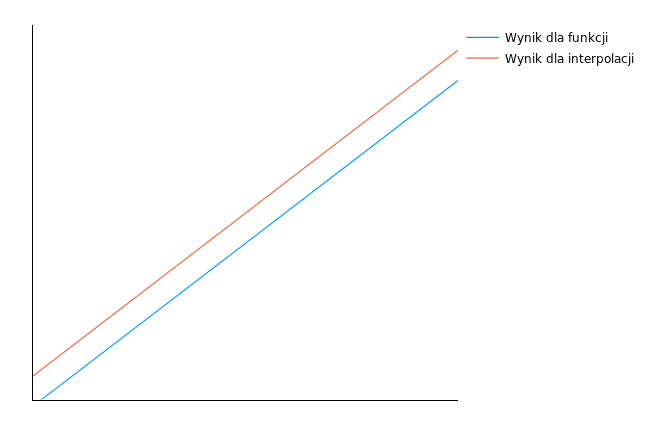
\includegraphics[scale=0.5]{5/5zoom.png}\\
\end{center}
 Jeśli bardzo przybliżymy to zauważymy pewne różnice i wraz ze wzrostem n są one coraz mniejsze.
\end{homeworkProblem}


%----------------------------------------------------------------------------------------
%	PROBLEM 6
%----------------------------------------------------------------------------------------

% To have just one problem per page, simply put a \clearpage after each problem

\begin{homeworkProblem}
%opis problemu
\subsection{Opis problemu}
Zadanie polegało na narysowaniu wykresów poprzez skorzystanie z funkcji napisanej w Zadaniu 4 dla podanych przypadków:
\begin{enumerate}
\item $|x|$, [-1,1], n= 5, 10, 15
\item $\frac{1}{1+x^2}$, [-1,1], n= 5, 10, 15
\end{enumerate}
%opis rozwiązania
\subsection{Opis rozwiązania}
Korzystam z uprzednio napisanej funckji poprzez uruchomienie jej z podanymi parametrami.
%wyniki
\subsection{Wyniki}
\begin{center}
Wynik dla podpunktu 1. z n=5\\
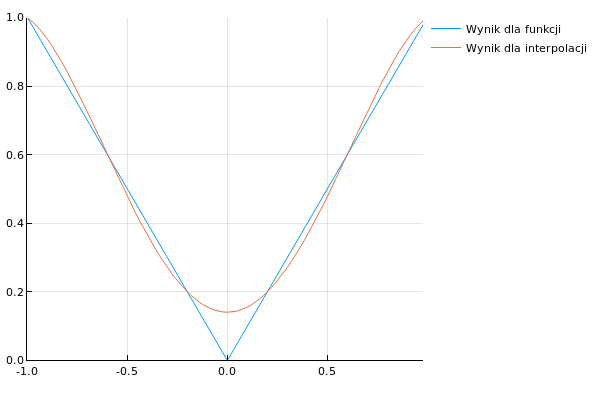
\includegraphics[scale=0.5]{6/a5.png}\\
Wynik dla podpunktu 1. z n=10\\
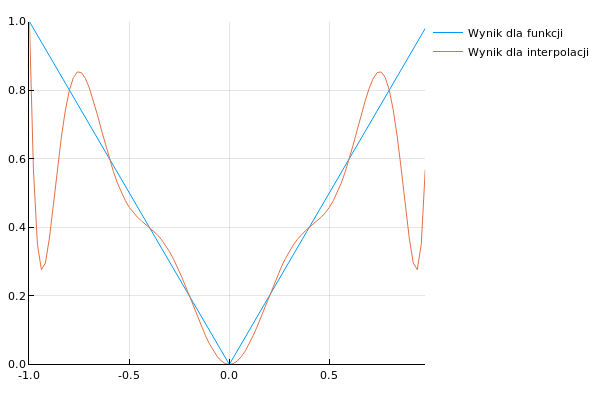
\includegraphics[scale=0.5]{6/a10.png}\\
Wynik dla podpunktu 1. z n=15\\
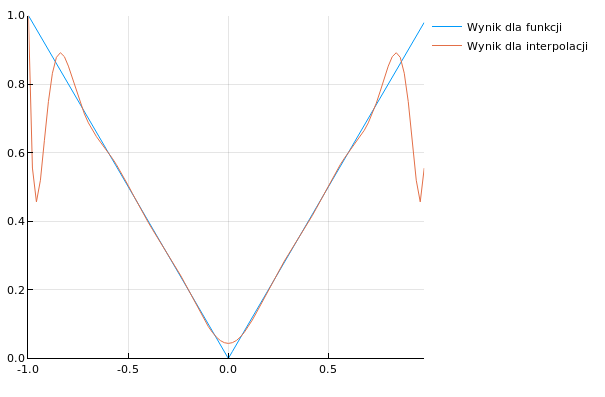
\includegraphics[scale=0.5]{6/a15.png}\\
Wynik dla podpunktu 2. z n=5\\
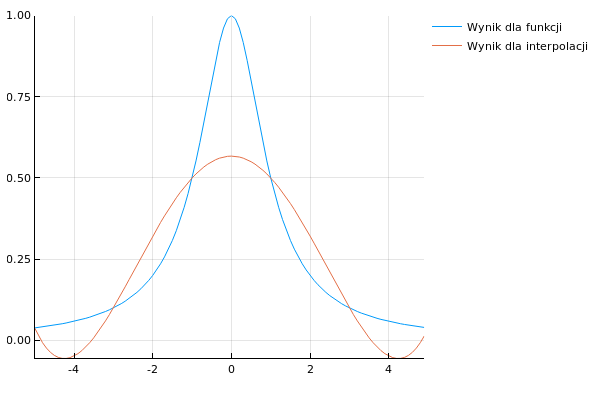
\includegraphics[scale=0.5]{6/b5.png}\\
Wynik dla podpunktu 2. z n=10\\
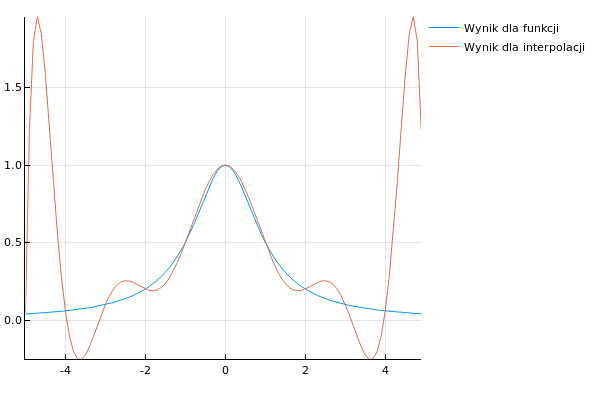
\includegraphics[scale=0.5]{6/b10.png}\\
Wynik dla podpunktu 2. z n=15\\
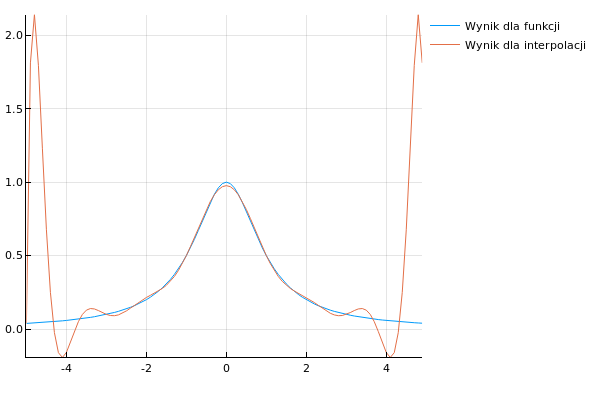
\includegraphics[scale=0.5]{6/b15.png}\\
\end{center}
%wnioski
\subsection{Wnioski}

W pierwszym jak i w drugim przypadku, łatwo da się zauważyć, że niedokładność wielomianu interpolacyjnego są dość znaczące i rosną wraz z n. Wynika to z faktu, że węzły są rozłożone równomiernie i na końcach przedziału zachodzi efekt Rungr'go. Przez to da się zaobserwować niechcianą "falę". Aby uniknąć tego problemu należałoby zwiększyć ilość węzłów na krańcach przedziału, sprawiając, że węzły nie byłyby już równoodległe od siebie. Do wyznaczania takich węzłów mogłby nam posłużyć zera wielomianu Czebyszewa. 

\end{homeworkProblem}



%----------------------------------------------------------------------------------------

\end{document}